\documentclass[tikz,border=5mm]{standalone}
\usetikzlibrary{shapes.geometric, arrows.meta}

\tikzset{
    block/.style = {rectangle, draw, fill=blue!20, text width=4em, text centered, rounded corners, minimum height=4em},
    line/.style = {draw, -Stealth, thick}
}

\begin{document}
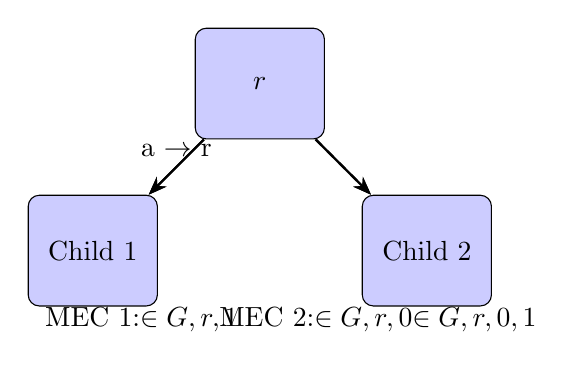
\begin{tikzpicture}[node distance=3cm]
    % Nodes
    \node[block] (root) {\( r \)};
    \node[block, below left of=root] (child1) {Child 1};
    \node[block, below right of=root] (child2) {Child 2};

    % Edges for MEC 1
    \path[line] (root) -- node[above] {a $\rightarrow$ r} (child1);
    \path[line] (root) -- (child2);

    % Edges for MEC 2
    \path[line] (root) -- (child1);
    \path[line, dashed] (root) -- (child2); % Undirected edge

    % Labels for MEC conditions
    \node[below of=root, xshift=-1.5cm] {MEC 1: \\ \(\in \setofMECs{G, r, 1}\)};
    \node[below of=root, xshift=1.5cm] {MEC 2: \\ \(\in \setofMECs{G, r, 0}\) \\ \(\in \setofMECs{G, r, 0, 1}\)};
\end{tikzpicture}
\end{document}